\section{Data Collected}

The MARATHON experiment ran from January through April of 2018 in Hall A at JLab. During the experiment the HRSs were used in ``inclusive'' mode, that is each spectrometer was making an independent measurement. Throughout the discussion of the analysis each measurement by an HRS is referred to as a ``kinematic''. To switch between kinematics the LHRS was rotated around the target to different angles. The RHRS was parked at the highest angle kinematic for the entirety of the experiment since that kinematic had a very slow event rate.

\begin{table}[h]
\begin{center}
\begin{tabular}{|l|l|l|l|l|}
\hline
\textbf{Kinematic} & \textbf{E$^\prime$} (GeV/$c$) & \textbf{Angle} ($\degree$) & \textbf{Central $x$} &  \textbf{No. of Iterations} \\
\hline
\hline
0 & 3.1 & 16.9$\degree$ & 0.199 & 1 \\ \hline
1 & 3.1 & 17.577$\degree$ & 0.218 & 1 \\ \hline
2 & 3.1 & 19.115$\degree$ & 0.257 & 1 \\ \hline
3 & 3.1 & 20.578$\degree$ & 0.298 & 1 \\ \hline
4 & 3.1 & 21.93$\degree$ & 0.338 & 1 \\ \hline
5 & 3.1 & 23.213$\degree$ & 0.378 & 1 \\ \hline
7 & 3.1 & 25.594$\degree$ & 0.46 & 2 \\ \hline
9 & 3.1 & 27.778$\degree$ & 0.538 & 2 \\ \hline
11 & 3.1 & 29.917$\degree$ & 0.62 & 2 \\ \hline
13 & 3.1 & 31.732$\degree$ & 0.70 & 2 \\ \hline
15 & 3.1 & 33.562$\degree$ & 0.78 & 3 \\ \hline
16 & 2.9 & 36.12$\degree$ & 0.82 & 2 \\ \hline
\end{tabular}
\caption{This table describes the key variables that define each kinematic.}
\label{tbl:kins}
\end{center}
\end{table}

For all kinematics the LHRS momentum was set to $3.1$ GeV/$c$. The RHRS momentum was set to $2.9$ GeV/$c$ due to limitations of the dipole magnet. The kinematics are numbered based on the originally proposed kinematic settings. Due to time limitations, not every kinematic was measured. During the data taking the $x$ and $Q^2$ values of the data were studied and it was found that there was sufficient overlap between kinematics without the skipped kinematics. Plots showing this overlap can be seen in Figure \ref{fig:kin_plots}. A few kinematics were measured more than once when the run period was extended. Individual iterations of a kinematic are treated as independent measurements for the sake of analysis. Table \ref{tbl:kins} shows the variables that define each kinematic.

\begin{figure}[h]
\begin{center}
	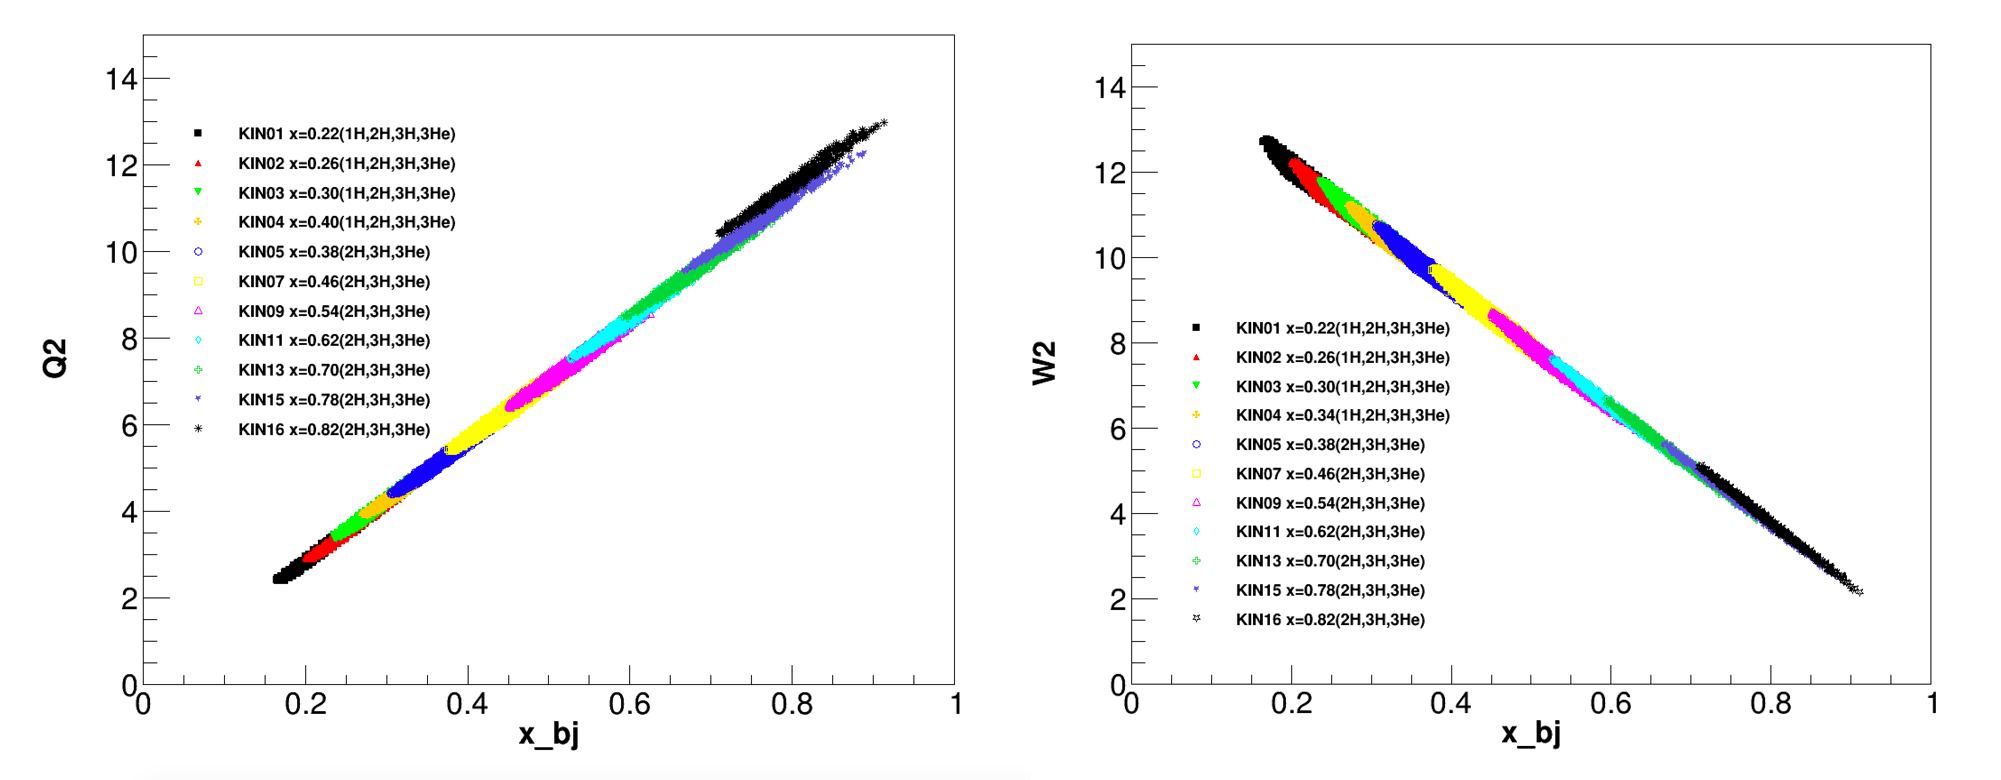
\includegraphics[width=\textwidth]{./analysis/fig/kin_plots.png}
	\caption{These plots show the $x$, $Q^2$, and $W^2$ coverage of all of the MARATHON kinematics. Each kinematic overlaps with the previous and successive kinematic, giving complete coverage of the proposed range of the experiment.\cite{Tong}}
	\label{fig:kin_plots}
\end{center}
\end{figure}

\section{Analysis Outline}
\label{sec:analysis_outline}
This chapter will go over the analysis of the data collected in the MARATHON experiment. Specifically examined are the cuts and corrections that go into this calculation as well as the calibrations performed to make the measurements accurate. An outline of the analysis process is as follows:
\renewcommand{\labelenumii}{\roman{enumii}.}
\begin{enumerate}
	\item For each run:
	\begin{enumerate}
		\item Apply cuts to data
		\item Calculate the electron yield and bin data in $x$
		\item Apply livetime correction
		\item Apply target boiling correction
		\item Calculate target boiling uncertainty
		\item Calculate beam charge and add it to the kinematic charge total
	\end{enumerate}
	\item For each kinematic:
	\begin{enumerate}
		\item Sum the yields from all runs in the kinematic
		\item Apply charge normalization
		\item Sum the target boiling uncertainties and apply them to the data
		\item Drop the first and last bins as they are near the edge of the acceptance
	\end{enumerate}
	\item For production of a ratio, the kinematic yields for two targets are divide ($^3$He and $^2$H in the case of this thesis)
	\item Combine all kinematics by weighted average, weighted by uncertainty
	\item Apply remaining corrections:
	\begin{enumerate}
		\item Endcap Contamination subtraction
		\item Charge Symmetric Background subtraction
		\item Target energy loss correction
		\item Coulomb correction
		\item Radiative Corrections
		\item Bin centering correction
	\end{enumerate}
\end{enumerate}
This analysis procedure will yield the $\nicefrac{F_2^{^3\textrm{He}}}{F_2^{^2\textrm{H}}}$ structure function ratio. From there, the A=3 isoscalar EMC ratio can be extracted by applying an isoscalar correction. Also, the $\nicefrac{F_2^n}{F_2^p}$ nucleon structure function ratio can be extracted using the methodology described in Section \ref{sec:F2ratio}.

\section{Yield and Yield Ratio Calculation}

The MARATHON experiment measured yield ratios. This method allows us to cancel many systematics that would otherwise plague a full cross section analysis. By taking data for each target at the same kinematics, acceptance effects are identical. This data taking technique means that with reasonable acceptance cuts, a ratio of target yields is wholly equivalent to the ratio of cross sections.

Calculating the the yield ratios requires first calculating the yield for each target. The yields calculated are binned in Bjorken $x$. The bins are 0.03 wide. The bin centers are defined by segmenting the range of 0 to 0.99 by 0.03 (i.e. the bins are centered at 0.015, 0.045, 0.075, etc.). The charge-normalized yield, $Y$, of each bin is calculated using this simple equation:
\begin{equation}
	Y = \frac{\text{Counts}}{\text{Scattering Centers} \cdot \text{Charge}} \cdot \text{Corrections}
	\label{eqn:yield}
\end{equation}
Here ``Counts'' are the number of electrons measured that pass the cuts placed on the data and fall into that bin, ``Scattering Centers'' are the number of nucleons in the target (calculated from the target thickness, mass, and mass number $A$), and ``Corrections'' are physics or systematic effects that are otherwise unaccounted for in the data. Dividing by the ``Charge'' in each kinematic, gives us the ``Charge-Normalized Yield'', that is the expected electron count for each unit of charge incident on the target.

As described in Section \ref{sec:analysis_outline}, the charge-normalized yield is calculated for each target on a per-kinematic basis. For each kinematic, the target ratios, $R$, are then calculated. This is done simply by dividing the two yields and propagating the associated uncertainties. The equations for taking the ratio are:
\begin{equation}
	R = \frac{Y_{^3\text{He}}}{Y_{^2\text{H}}}
\end{equation}
\begin{equation}
	\sigma_{R} = R\sqrt{\left(\frac{\sigma_{^3\text{He}}}{Y_{^3\text{He}}}\right)^2 + \left(\frac{\sigma_{^2\text{H}}}{Y_{^2\text{H}}}\right)^2}
\end{equation}

Once the per-kinematic yield ratios are calculated, each kinematic has its edge bins dropped, that is the lowest and highest $x$ bin. This is because these bins are located at the edge of the acceptance of the spectrometer with low counting rates and large uncertainties. After this is done, all kinematics are combined through a weighted average. The ``weight'' is the uncertainty on the measurement in that bin. The equations for the weighted average are:
\begin{equation}
	\text{Average} = \frac{\sum\limits_{i} \frac{R}{\sigma^2_R}}{\sum\limits_{i} \frac{1}{\sigma^2_R}}
\end{equation}
\begin{equation}
	\sigma_\text{Average} = \frac{1}{\sum\limits_{i} \frac{1}{\sigma^2_R}}
\end{equation}
Once all corrections have been applied, this calculated weighted average is the final result for the yield ratio.

%\section{Calibrations}
%%\subsection{ADC Calibrations}

\subsection{Raster Calibration}
The raster is calibrated by defining a line that maps the raster current to positions at each BPM and the target. To do this, the slope and intercept of this line had to be determined. The slope corresponds to the conversion of raster current to position displacement. The intercept is then determined from the central position that the beam is displaced from. This section will be a general presentation of the techniques used to calibrate the raster. For a more in-depth discussion of how the raster was calibrated, see Appendix \ref{raster_appendix}.

For the horizontal raster, this was done by optimizing the reconstructed z-vertex on the target. When properly calibrated, there should be no correlation between the horizontal raster and the z-vertex. Linear interpolation between two ``bad'' calibrations is a simple way to determine the correct calibration slope.

The veritcal raster could be calibrated in a similar way by minimizing the correlation between the vertical raster and a known momentum phenomena (i.e. a $W^2$ peak). Unfortunately, such a feature does not exist within the kinematics of MARATHON data. The vertical calibration was determined using the carbon hole target. The hole is known to be $2mm$ diameter. By using the raster data, the hole can be fit in order to determine the vertical calibration slope.

The intercepts are determined by looking at the mean BPM position readings and projecting these to the target. This position will correspond to the mean value of the rasters as well. Using the beam position, raster current, and calibration slope the calibration intercept can easily be determined.


\section{Cuts}
When analyzing the data, cuts must be applied to give a set of ``good electrons''. Cuts are a defined set of conditions that must be met by an event to be classified as ``good''. In this analysis, the cuts can be classified in two categories: Particle Identification and Acceptance. Particle Identification cuts are used to ensure that all events being studied are electrons. Acceptance cuts are used to ensure that all events passed through areas of the spectrometer that are well constrained by the spectrometer optics.

\subsection{Particle Identification}

Particle Identification (PID) cuts are applied to the detectors in the HRSs. The first PID cut is referred to as the ``Trigger 2'' cut. This cut requires that an event fires Trigger 2 (Trigger 5 for the RHRS) which is the (S0 \&\& S2) \&\& Cherenkov trigger. This cut requires that S0 and S2 fire, which will ensure proper event timing and tracking. Ensuring that the Cherenkov fires is the first step to limiting the events to electrons. As described in Section \ref{sec:cer}, the Cherenkov will, in most cases, only fire for electrons due to the 4.8 GeV/\textit{c} momentum threshold for pion detection.

The next cut is the ``1-Track'' cut. This cut requires that an event must have only one track through the spectrometer associated with it. A single track assures that the event corresponds to a single electron. When multiple tracks are present, there is a risk that tracking and spectrometer readings will be incorrect.

There is a cut placed on the $W^2$ of an event. The goal of MARATHON is to measure the DIS cross section ratios. A cut on $W^2$ must be placed in order to ensure that all events are from the DIS region and to reject events that originate from Resonance scattering. This cut is placed for $W^2>3$  GeV$^2$/\textit{c}$^4$.

A cut is placed on the Cherenkov signal. This cut is placed on the ADC spectrum of the Cherenkov. For the LHRS the cut is at 1500; the cut is placed at 2000 for the RHRS. While the Cherenkov will generally only fire for electrons, there are a small number of high momentum pions that are capable of creating a signal. The high momentum threshold for pions means that any pions that do create a signal will create a very small signal. This can be seen in Figure \textbf{blah}. By placing this cut, the pion peak is completely removed while the electron peak is nearly completely allowed to pass.

The final PID cut is on the ratio of the energy of the particle to the momentum of the track ($E/p$). For electrons, which have a low mass compared to the energy scale of the experiment, the $E/p$ is expected to be approximately 1. Any particle of larger mass that passes the ``Trigger 2'' cut (and thus created a Cherenkov signal) will have an $E/p$ value significantly smaller than 1. In order to eliminate these non-electron events a cut on $E/p$ is placed at $0.7$ for both arms. This spectrum can be seen in Figure \textbf{blah}.

\subsection{Acceptance}

Acceptance cuts are placed on the kinematic region that the spectrometer is sensitive to. These cuts are applied to the tracking variables ``Target $\phi$'', ``Target $\theta$'', and ``$\delta p$''. Target $\phi$ is a measure of the rotation in the plane of the hall floor. The value is the angular displacement from the central angle of the spectrometer. Target $\theta$ is the vertical angular displacement of the scattered electron. $\delta p$ is the deviation of the momentum of the scattered electron from the central momentum of the spectrometer. The RHRS also has a cut placed on the focal plane. These cuts are defined by looking at the acceptance of the spectrometer. Examining the acceptance of each spectrometer, cuts were placed around the area where the events were concentrated. The areas where events ``fell off'' were considered to be outside of the acceptance of the spectrometer. This is also how the focal plane cuts were determined for the RHRS.

The other acceptance cut that is applied is to the target length. This cut is applied to the ``z-Target'' value of an event, where the event happened in the target along the axis of the beamline. This cut is used in order to minimize the amount of Endcap Contamination events that need to be corrected for. The cut is defined on a kinematic-by-kinematic basis, with higher kinematics having more of the target length allowed to pass the cut due to a smaller endcap contribution to the overall event rate. These cuts are defined in Table \ref{tbl:ztar}.

\begin{table}
\begin{center}
\begin{tabular}{|c|c|}
\hline
\textbf{Kinematics} & \textbf{z-Target Acceptance (m)}\\
\hline\hline
0 - 4 & $-0.08$ - $0.1$ \\ \hline
5 - 7 & $-0.09$ - $0.1$ \\ \hline
9 - 11 & $-0.095$ - $0.1$ \\ \hline
13 - 15 & $-0.1$ - $0.105$ \\ \hline
16 & $-0.105$ - $0.11$ \\ \hline
\end{tabular}
\caption{This table shows the range of the target, along the beam axis, that events are accepted from. This is done to minimize contamination from the endcaps of the targets.}
\label{tbl:ztar}
\end{center}
\end{table}

\section{Corrections}

\subsection{Target Boiling}
\label{sec:boiling}

Reference Sheren and Natalie paper.

Localized heating from the beam causes changes to the gas density of the target. The target does not actually boil, but the standard nomenclature for a change in target density is "boiling". By modulating the gas density, the incident beam sees a variable target thickness. This in turn affects the yield calculation.

This effect scales with the current that is on the target. We make this correction run-by-run using the average current during beam-on time during the run. This method was chosen because the average current is near constant over the coarse of a single run and the effect is approximately linear for small deviations in current. It was found that the change in density settles very quickly, so it is unnecessary to take into account beam ramp-up after beam trips.

To determine the correction, a dedicated set of runs was taken with the Left HRS spectrometer at $16.8\degree$ and $3.1GeV$. The data was taken at varying currents in order to assess the affect of the beam current on the normalized yield. By applying nominal event cuts to this data, the normalized yield was calculated. 

To determine the density correction, the normalized yields were plotted versus the beam current for that measurement. The data was then fit with a quadratic polynomial. The fit was constrained to require a correction of $1$ (no correction) at a current of $0 \mu A$.

\begin{figure}
	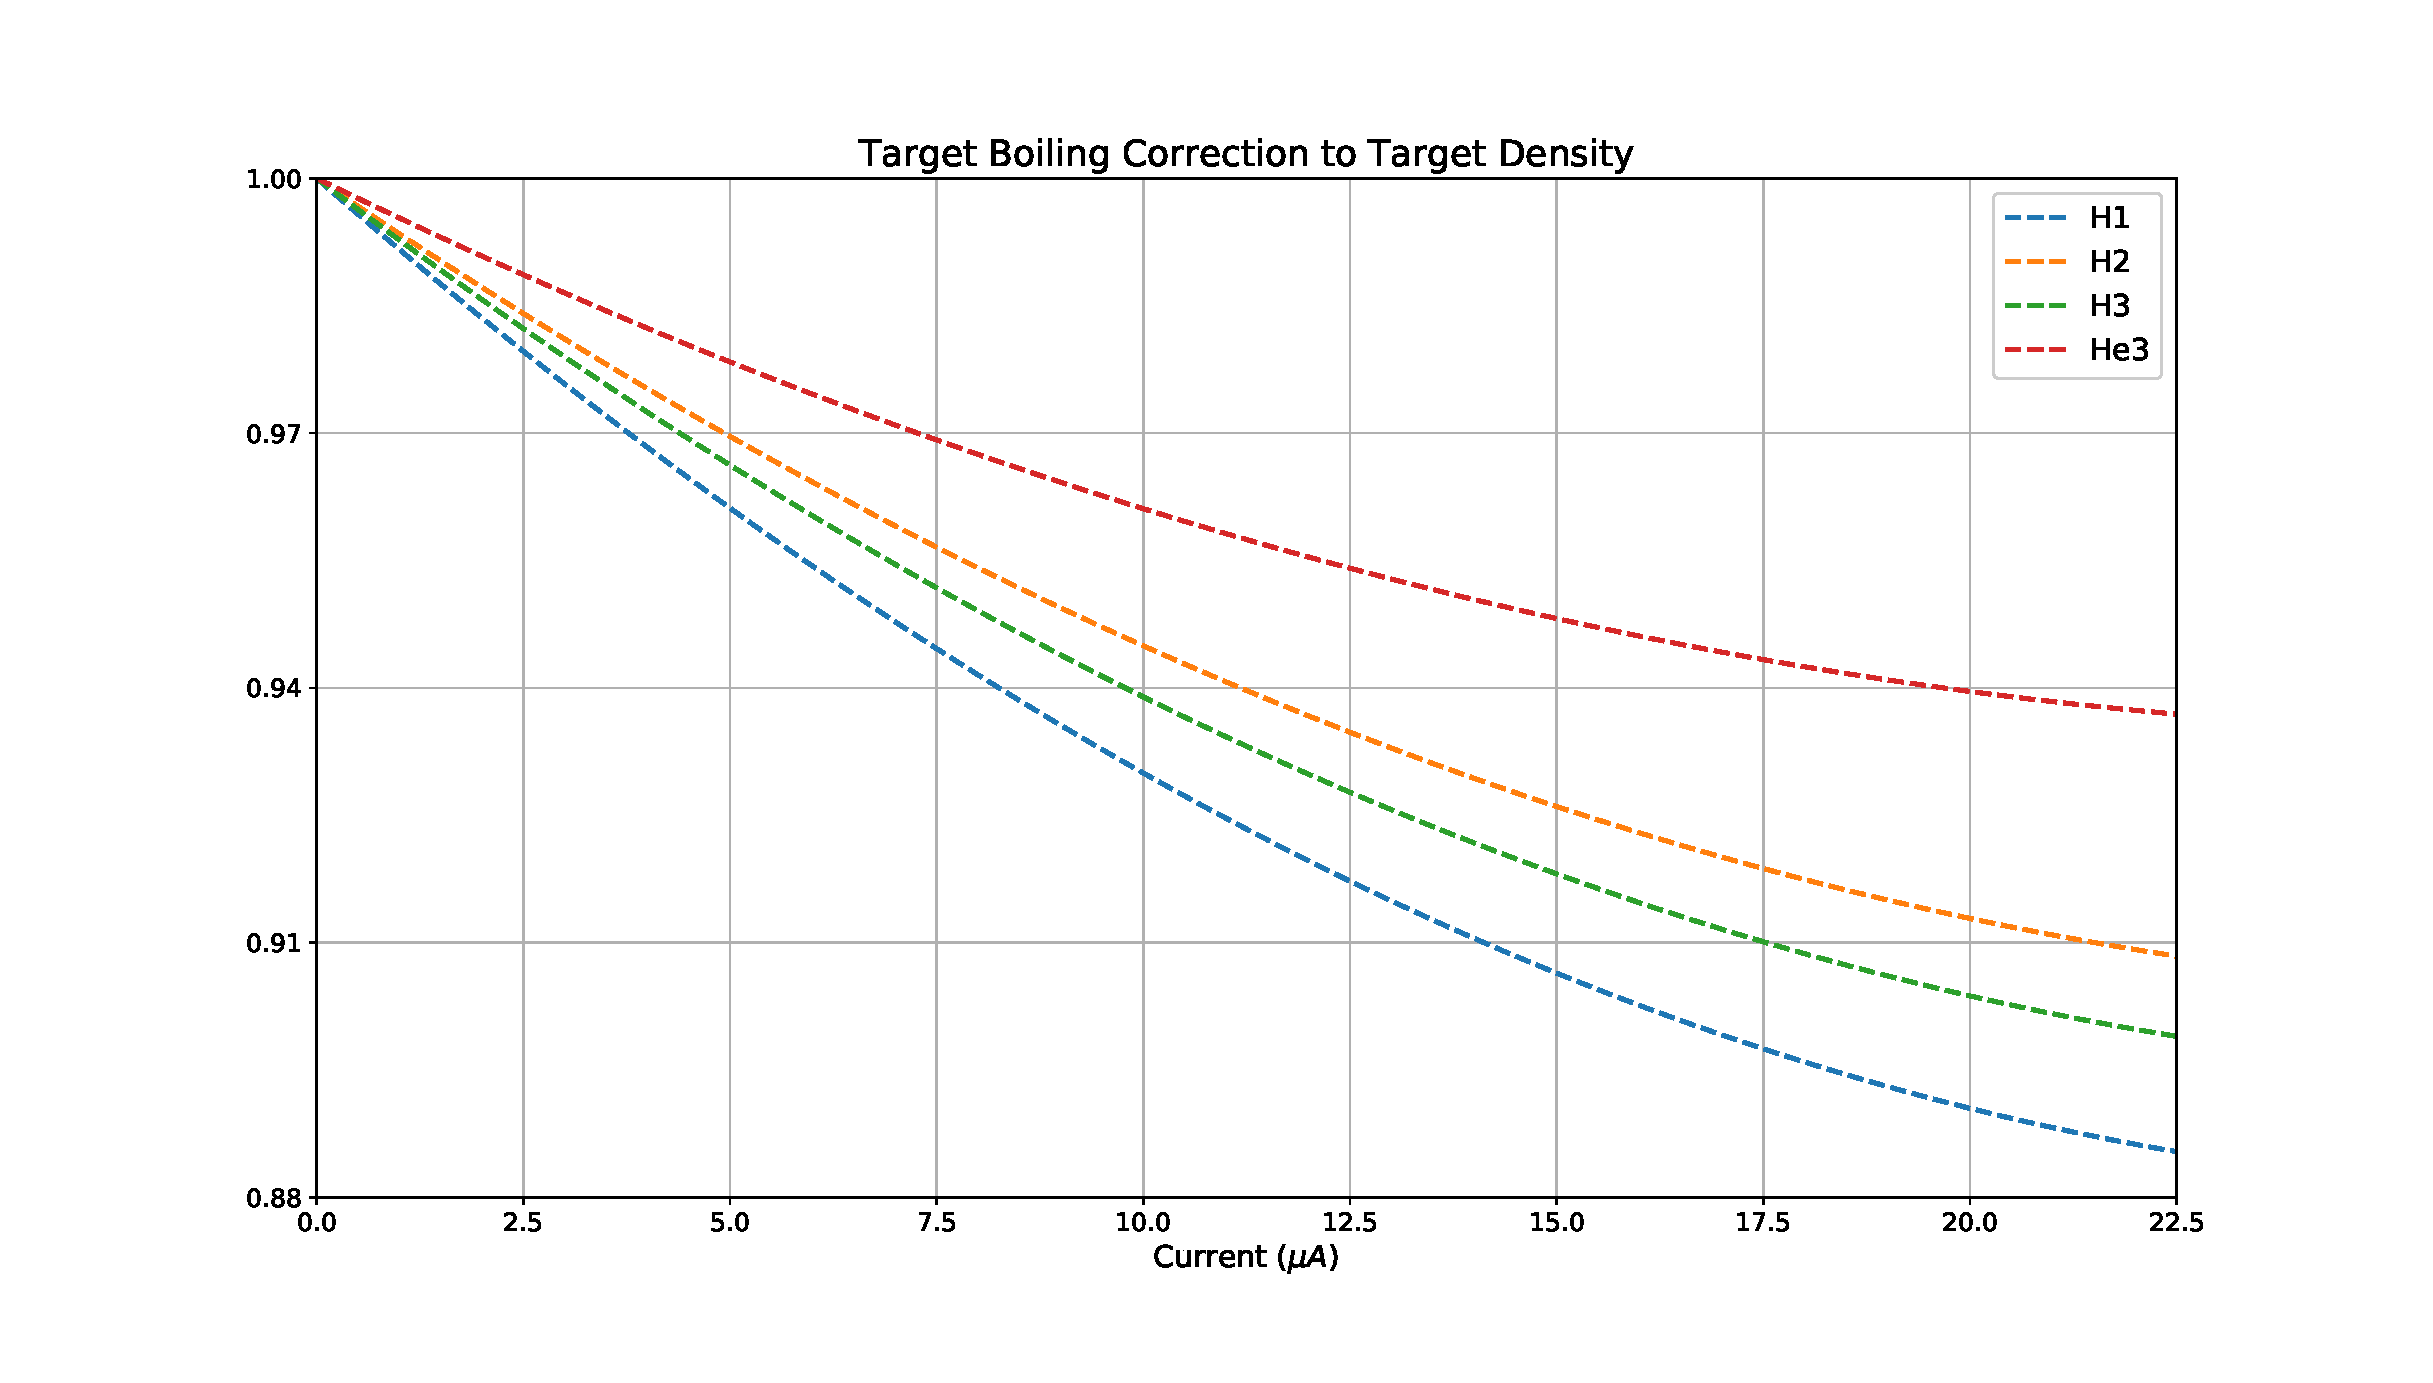
\includegraphics[width=\textwidth]{./analysis/fig/boil_cor.eps}
	\caption{Beam heating effects are manifested as a multiplicative correction to the target density}
	\label{fig:boilcor}
\end{figure}

\begin{figure}
	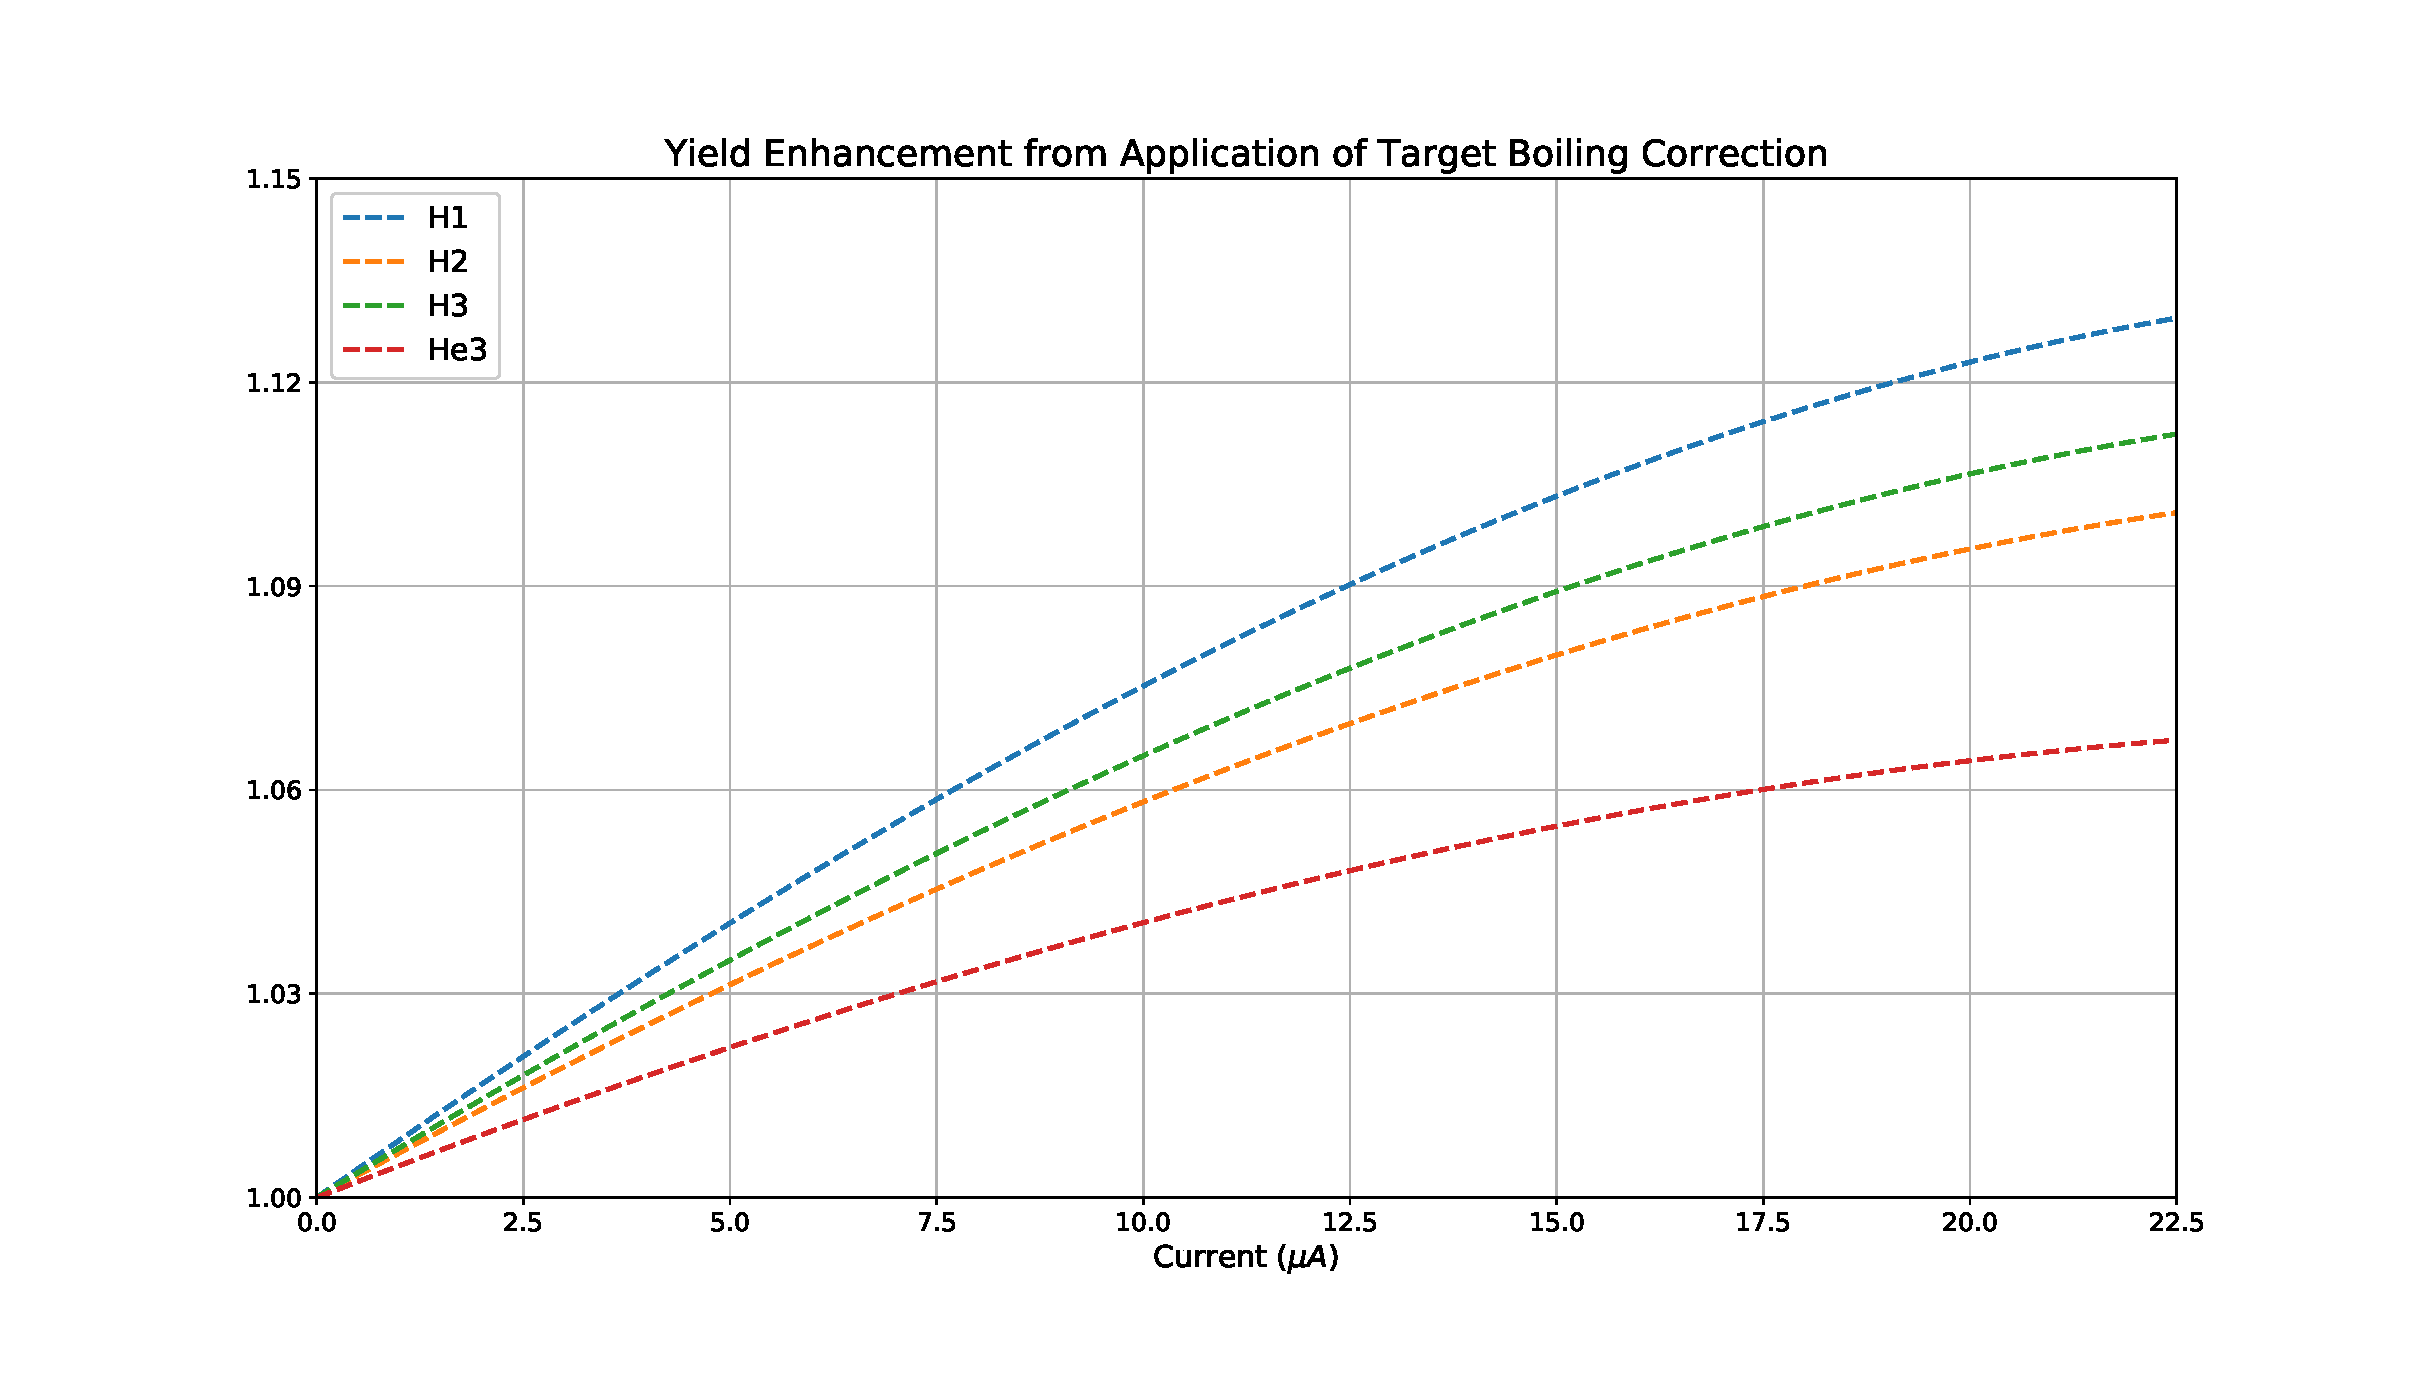
\includegraphics[width=\textwidth]{./analysis/fig/boil_yield_cor.eps}
	\caption{Target density corrections cause a multiplicative enhancement to the yield}
	\label{fig:boilyieldcor}
\end{figure}

\subsection{Target Endcap Contamination}
\label{sec:ecc}

All of our gas targets are stored in an aluminum cell. The thickness of the aluminum greatly exceeds the thickness of the gas and will sometimes contribute background that makes it past our cuts. To determine this contribution, we use an empty cell. The empty cell, being an exact replica of the gas target cells with a vacuum inside, allows us to approximately isolate the contribution of the cell walls to the data.

To determine this contribution, the empty cell is normalized to the target in question. This is done by.........

The data for the target in question and the normalized empty target are then binned in Bjorken x. Dividing the empty cell data by the gas target data then gives an approximation of the fractional contribution of the cell walls to the electron data. This fractional contribution can be the subtracted from the charge normalized yields to correct for the data coming from the endcaps.

\subsection{Charge Symmetric Background Subtraction}

As an inclusive scattering experiment, we are particularly susceptible to background from charge symmetric processes from the target. To study this background we reversed the polarity of the Left HRS to take positron data at several low Bjorken x kinematics.

Measuring the positron yield allows us to determine the proportion of electron events measured that were a result of pair production. This data was subject to the same cuts that are used on the electron data. It was noted that a significant $\pi^+$ contamination occurred for the positron data. The main pion peak was fit and then subtracted from the positron data.

These data were then binned by Bjorken x and fit with an exponential. 

Somethin somethin somethin... Provide x of bin and multiply by $1-\mathrm{curve}$.

\begin{figure}
	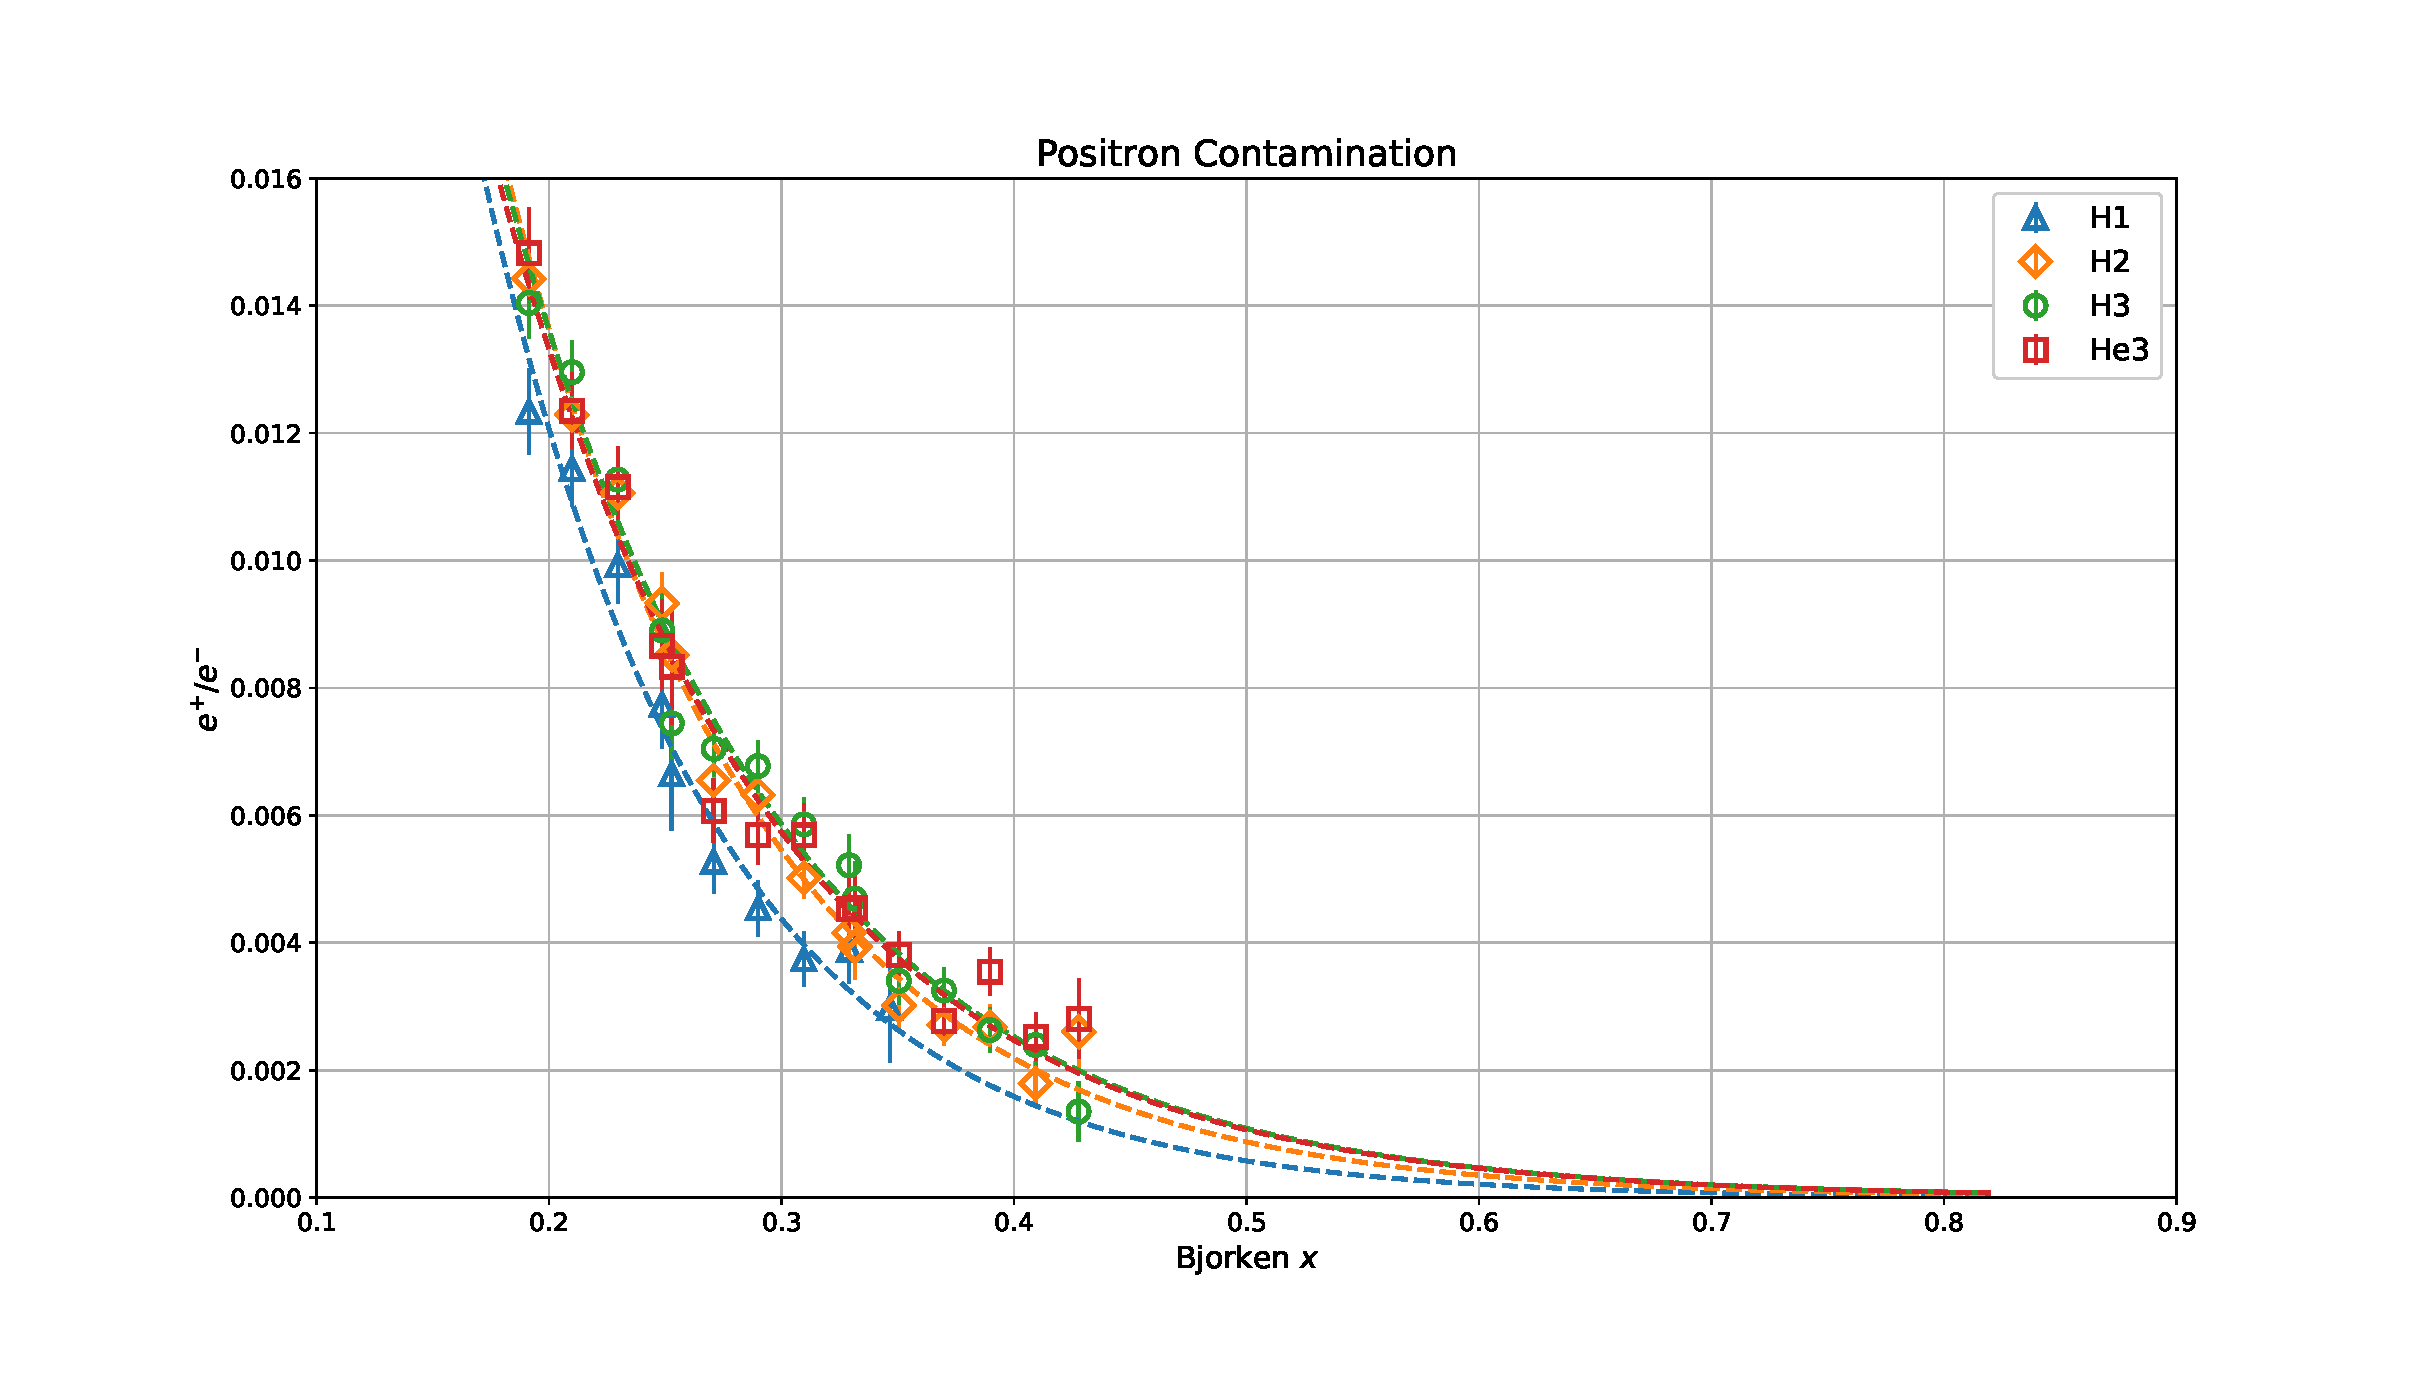
\includegraphics[width=\textwidth]{./analysis/fig/positrons.eps}
	\caption{Charge symmetric background correction}
	\label{fig:positrons}
\end{figure}

\subsection{Computer Deadtime Correction}

Our DAQ unable to be continuously taking data. While we can probabilistically determine the mean time spacing between events, in the real world events can deviate greatly from these means \textbf{because statistics}. Sometimes events will occur that are too close in time for our DAQ to record all of them. When deadtime becomes significant, we must correct for it.

An approximation of the computer deadtime was measured with our scalers. The trigger signals generated by the NIM electronics were copied and sent to both the Trigger Supervisor and a scaler unit. The Trigger Supervisor is subject to the computer deadtime event loss discussed here. The scaler unit simply increments a register when a trigger signal is received. The deadtime is defined on a run-by-run basis as:

\begin{equation}
DT = 1 - \frac{\Sigma \mathrm{Triggers_{TS}}}{\Sigma \mathrm{Triggers_{Scaler}}}
\end{equation}

A deadtime correction is applied on a run-by-run basis. The correction is defined as:

\begin{equation}
DT_{\mathrm{correction}} = \frac{1}{1-DT}
\end{equation}

\begin{figure}
	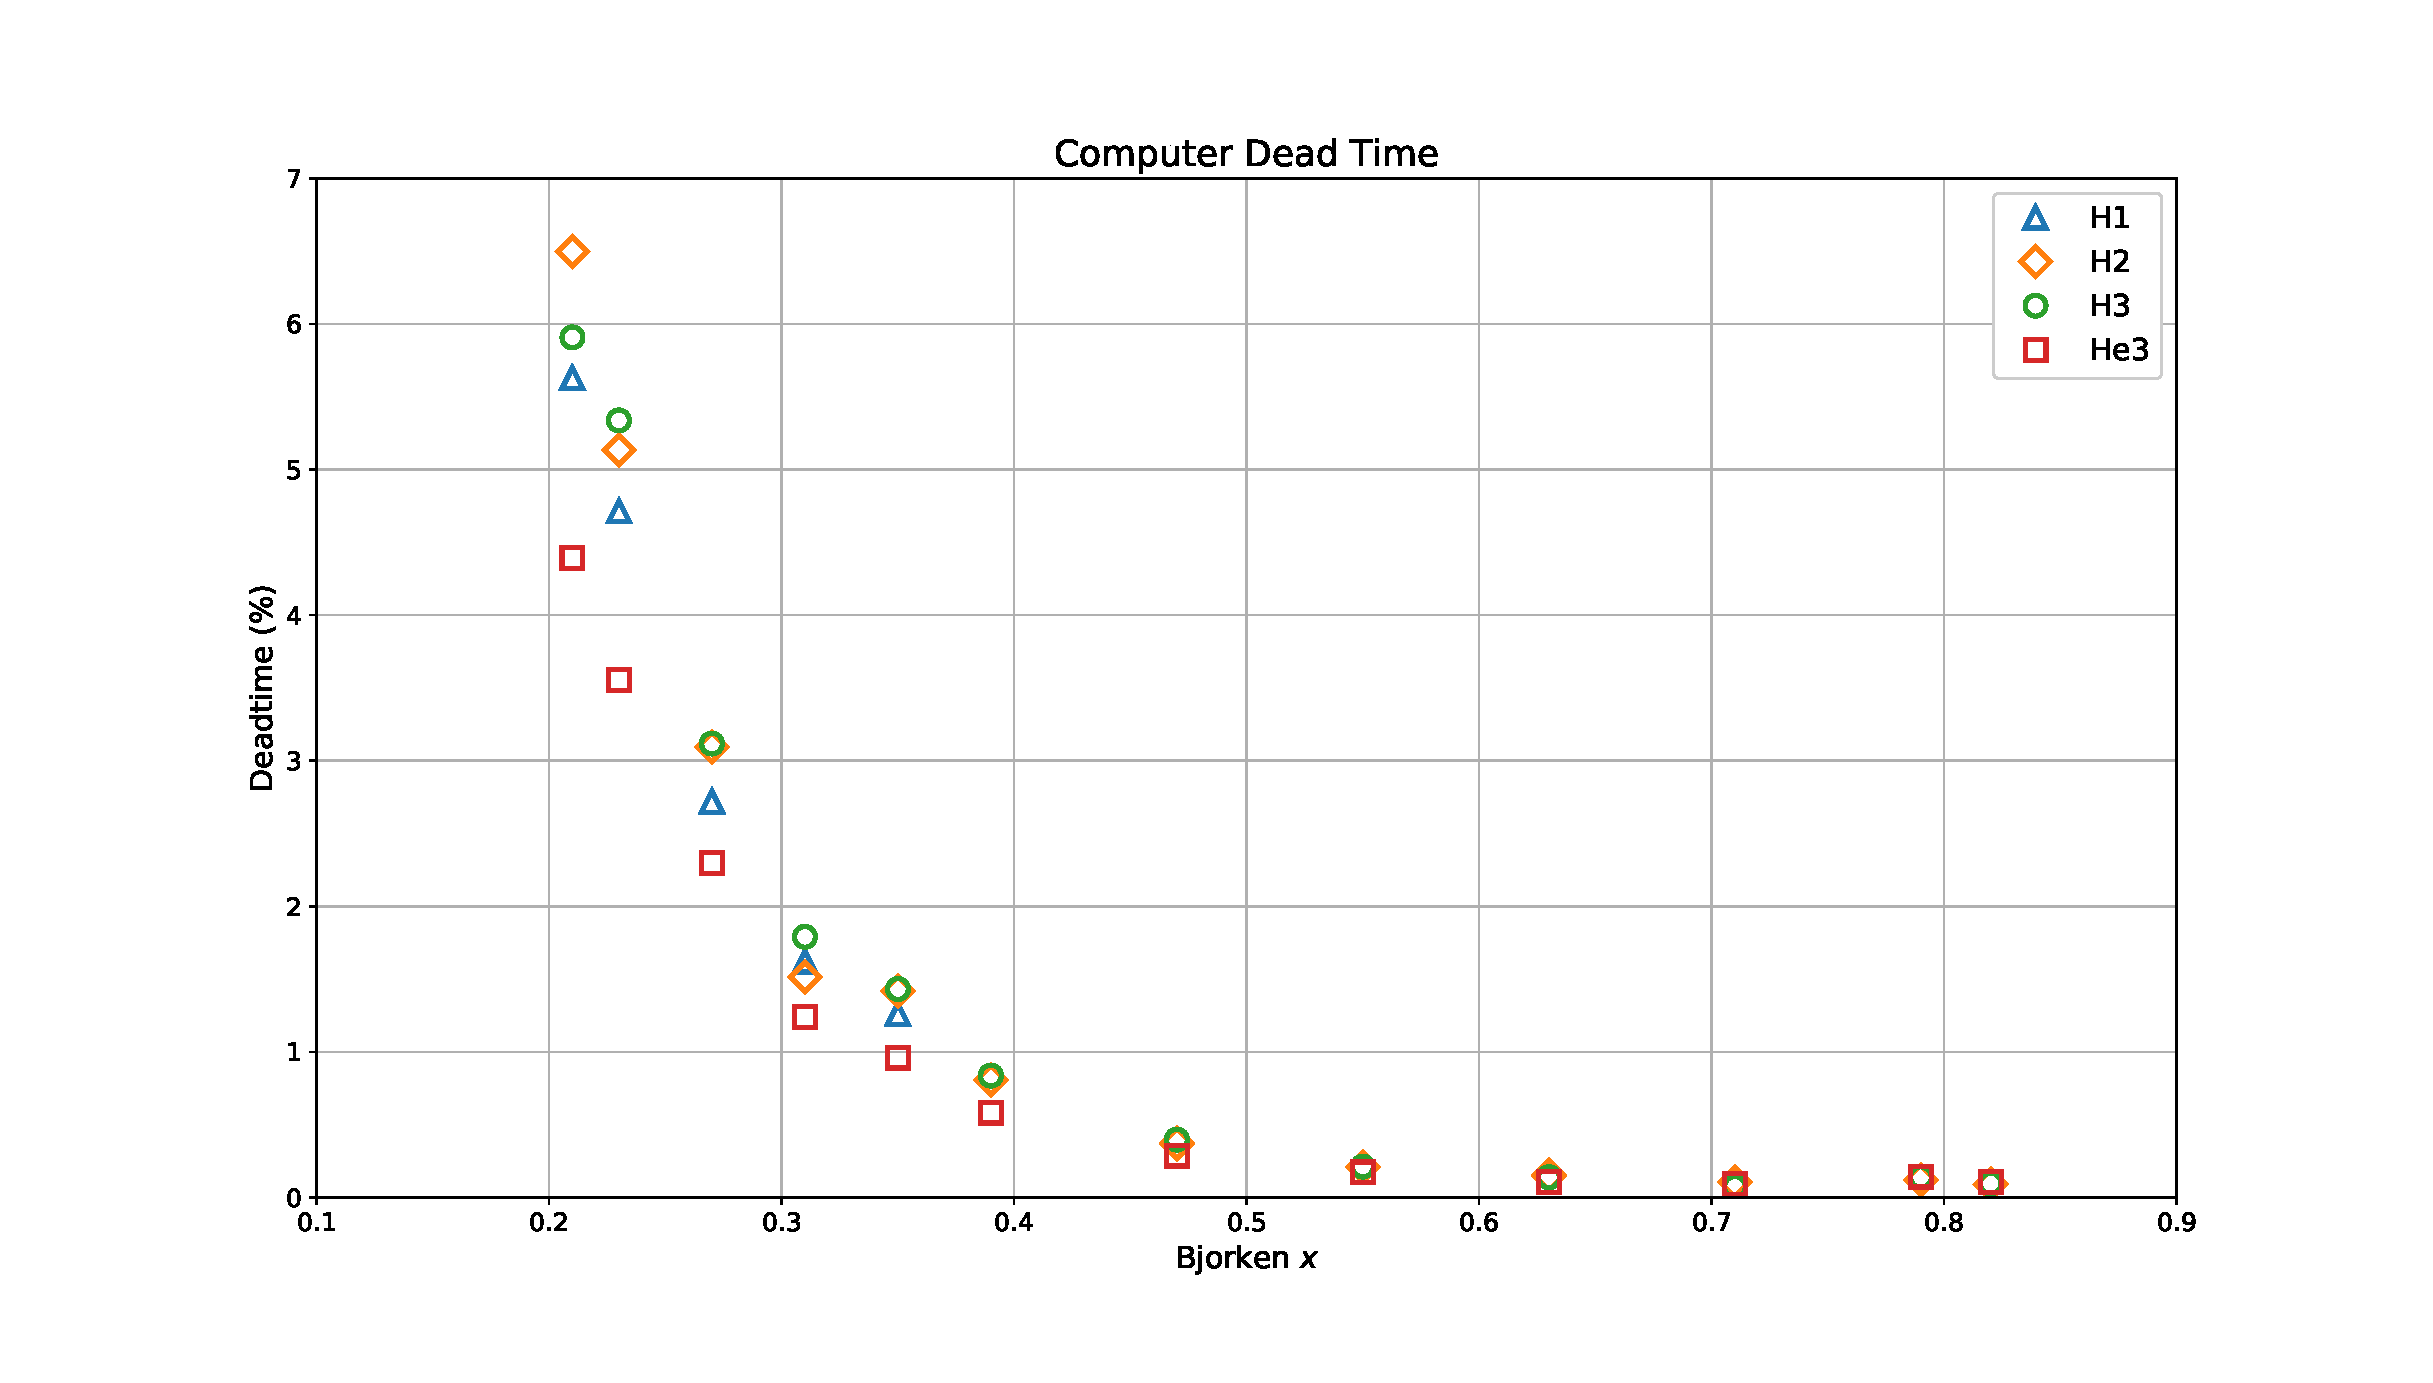
\includegraphics[width=\textwidth]{./analysis/fig/deadtime.eps}
	\caption{Deadtime per kinematic}
	\label{fig:deadtime}
\end{figure}

\subsection{Radiative Corrections}

\subsection{Isoscalar Corrections}

\subsection{Bin Centering Corrections}

\subsection{Coulomb Corrections}


